\chapter{Regulacja procesu}
	\label{ch:reg}
	
	\section{Implementacja NPL}
		\label{sec:NPL}
		
	\section{Strojenie NPL}
		\label{sec:stroj_NPL}
		
		\begin{figure}[h!]
			\centering
			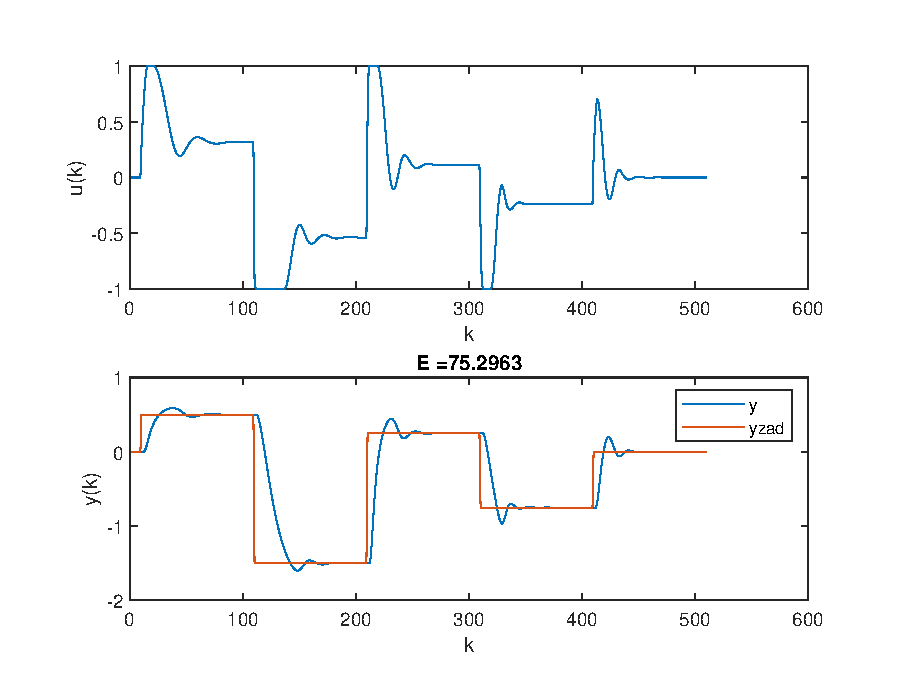
\includegraphics[width=\linewidth]{img/strojenieNPL_N_10_Nu_2_lam_1.eps}
			\caption{Działanie regulatora NPL z nastawami N=10, Nu=2, $\lambda$=1}
			\label{fig:NPL0}
		\end{figure}
		
		\begin{figure}[h!]
			\centering
			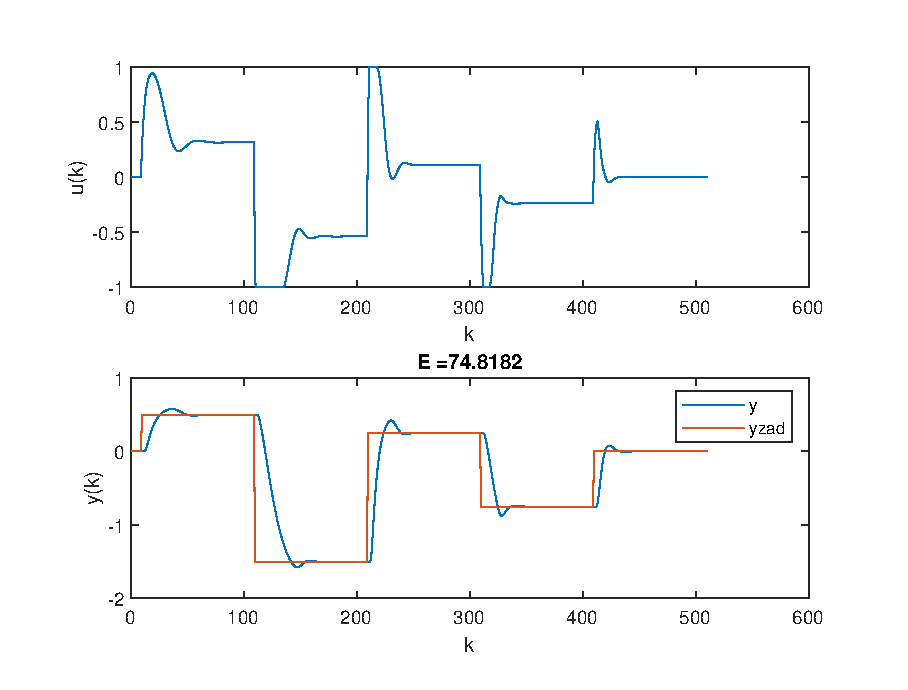
\includegraphics[width=\linewidth]{img/NPLN20.eps}
			\caption{Działanie regulatora NPL z nastawami N=20, Nu=2, $\lambda$=1}
			\label{fig:NPL1}
		\end{figure}
		
		\begin{figure}[h!]
			\centering
			\includegraphics[width=\linewidth]{img/NPLNu1.eps}
			\caption{Działanie regulatora NPL z nastawami N=20, Nu=1, $\lambda$=1}
			\label{fig:NPL2}
		\end{figure}
		
		\begin{figure}[h!]
			\centering
			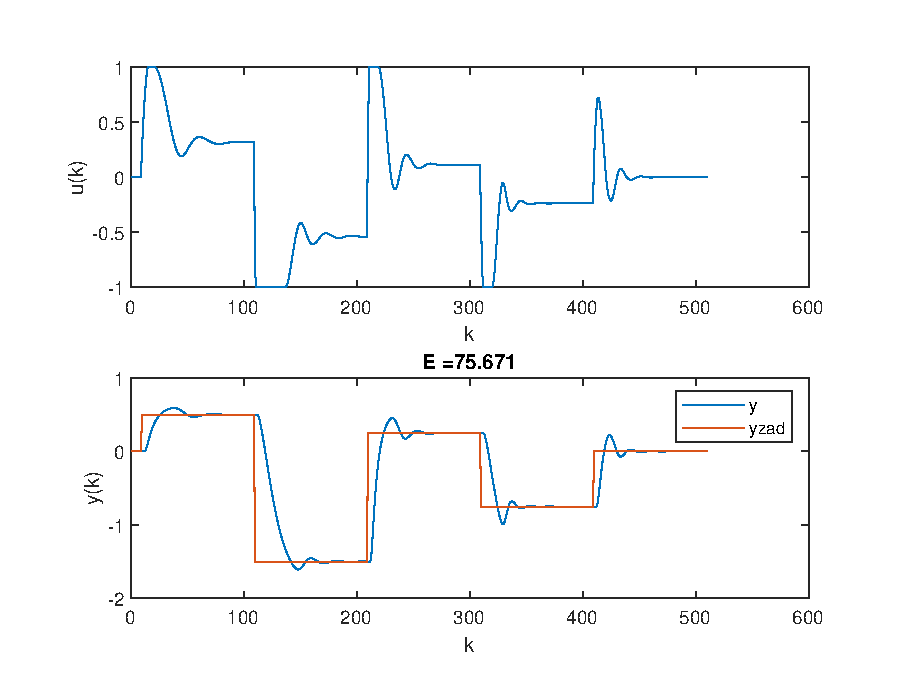
\includegraphics[width=\linewidth]{img/NPLNu3.eps}
			\caption{Działanie regulatora NPL z nastawami N=20, Nu=3, $\lambda$=1}
			\label{fig:NPL3}
		\end{figure}
		
		\begin{figure}[h!]
			\centering
			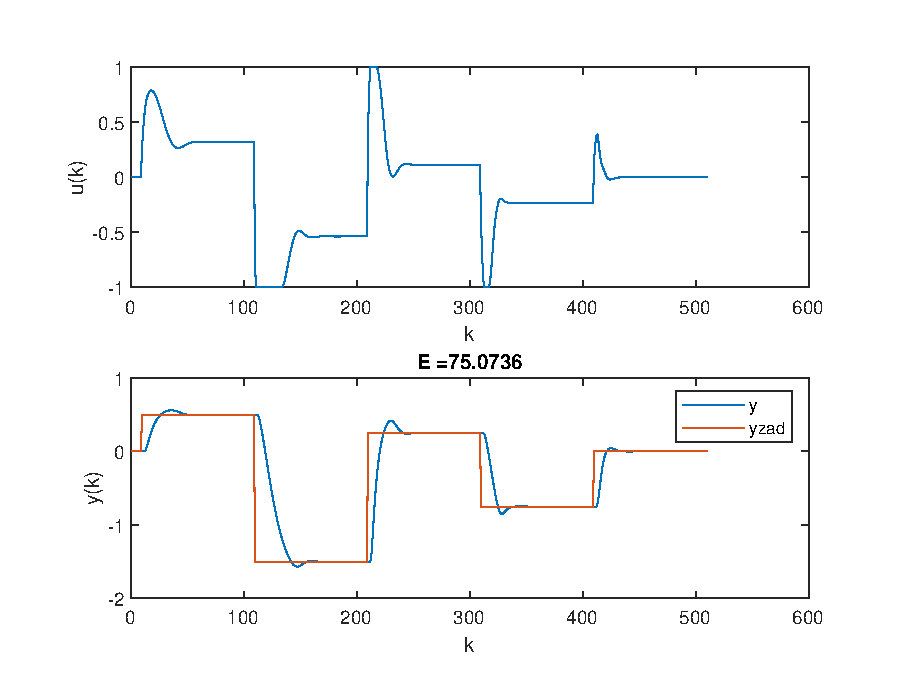
\includegraphics[width=\linewidth]{img/NPLlam2.eps}
			\caption{Działanie regulatora NPL z nastawami N=20, Nu=2, $\lambda$=2}
			\label{fig:NPL4}
		\end{figure}
		
		
	\section{GPC}
		\label{sec:GPC}
		
		\begin{figure}[h!]
			\centering
			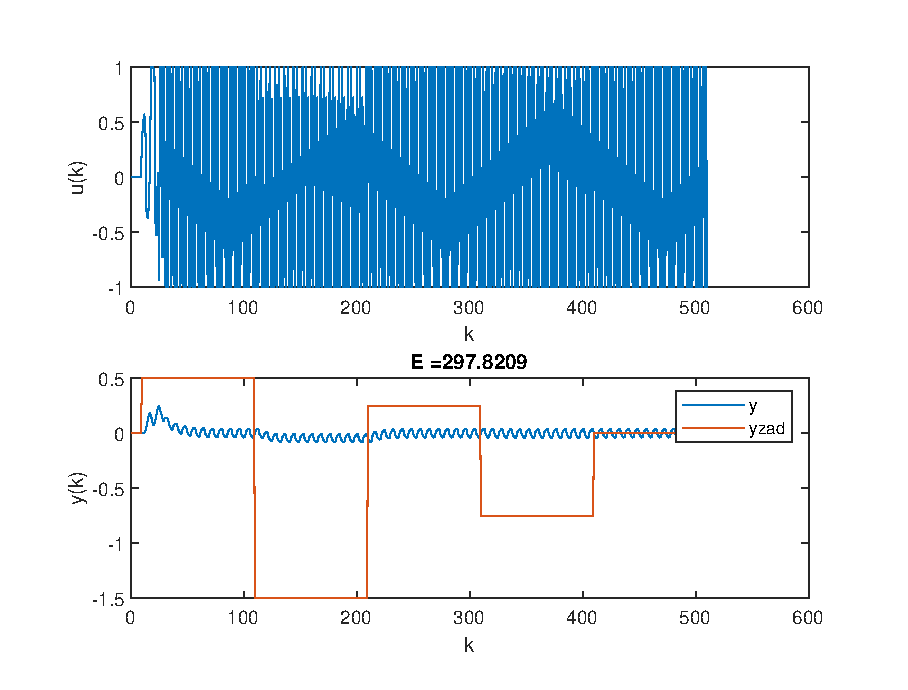
\includegraphics[width=\linewidth]{img/GPC.eps}
			\caption{Działanie regulatora GPC z nastawami N=20, Nu=2, $\lambda$=2}
			\label{fig:GPC}
		\end{figure}
		
		\begin{figure}[h!]
			\centering
			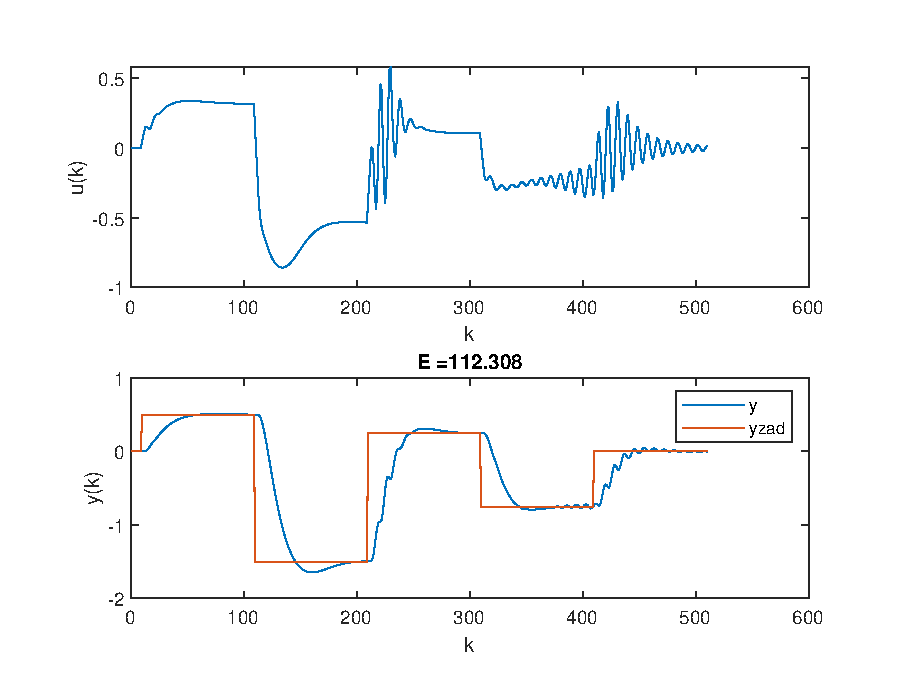
\includegraphics[width=\linewidth]{img/GPC100.eps}
			\caption{Działanie regulatora GPC z nastawami N=20, Nu=2, $\lambda$=100}
			\label{fig:GPC100}
		\end{figure}